\documentclass[11pt]{article}

\usepackage[T1]{fontenc}
\usepackage{amsmath,amssymb}
\usepackage{geometry}
\usepackage{graphicx}
\usepackage{hyperref}
\usepackage{microtype}
\usepackage{xcolor}

\geometry{margin=1in}
\graphicspath{{./}}
\hypersetup{colorlinks=true,linkcolor=blue!55!black,urlcolor=blue!55!black}

\newcommand{\code}[1]{\texttt{#1}}

\title{Mathieu1D Direct Finite Reduction\\
\large Calculation-facing technical report}
\author{Project Koios}
\date{\today}

\begin{document}
\maketitle

\begin{center}
\fbox{\begin{minipage}{0.92\linewidth}
\textbf{Status.} This report describes one retained, unsealed, illustrative finite
numerical execution.  Independent verification checks the exact result bytes and owns
the authenticated plot-data projection.  Neither the calculation nor this report
establishes continuum convergence, uncertainty quantification, material validation,
publication acceptance, or a sealed evidence package.
\end{minipage}}
\end{center}

\begin{abstract}
This report records a direct typed calculation of a one-dimensional Mathieu
Hamiltonian, independent reconstruction of its finite numerical channels, and two
figures rendered only from authenticated data.  The calculation compares finite
plane-wave and finite-difference representations, transforms one sampled band to a
complete finite hopping inventory, and evaluates declared symmetric hopping-range
truncations on separate training and evaluation coordinates.  The results concern the
specified finite representations and do not promote adjacent-representation changes
to continuum errors or uncertainties.
\end{abstract}

\section{Scientific question}

For the represented dimensionless Hamiltonian
\begin{equation}
  H=-\frac{d^2}{dx^2}+0.5\cos x,
  \qquad x\sim x+2\pi,
\end{equation}
how do the declared finite parent representations, the complete 64-point discrete
Fourier transform, and the finite symmetric hopping ranges behave on their fixed
coordinate inventories?

The calculation uses plane-wave cutoffs $3,5,7,9,11$ with cutoff $15$ as a finite
represented reference.  A separate periodic finite-difference route uses
$31,63,127,255$ points.  The lowest of three compared finite bands is sampled on a
64-point centered training mesh and a disjoint 257-point staggered evaluation mesh.
The declared maximum hopping ranges are $0,1,2,3,4,6,8$.  All energies are
nondimensional in the declared recoil-energy convention.

\section{Ownership and verification boundary}

Reusable source under
\code{ksdft2effmass.model\_systems.mathieu1d} owns typed configuration, calculation,
result, verification, authenticated projection, and rendering behavior.  The direct
calculation script composes existing plane-wave, periodic finite-difference, Fourier
transform, truncation, interpolation, diagnostic, and weighted least-squares owners.

The independent verifier does not call the producer analyzer.  It assembles dense
plane-wave fibers and sparse twisted finite-difference fibers directly, evaluates the
finite Fourier sums explicitly, and performs the weighted least-squares calculation
through a separate NumPy route.  It hashes the exact admitted result bytes and binds
the resulting digest to the plot-data projection.  Rendering reruns that verifier and
requires exact equality of both the verification aggregate and the authenticated
projection before publishing any figure.

\section{Complete authenticated view}

Figure~\ref{fig:complete} displays four finite-data channels: represented parent
refinement, the sampled evaluation band and selected finite-range reconstructions, the
complete finite-transform hopping magnitudes, and the declared range diagnostics.
Connected marks follow explicitly ordered finite inventories.  They do not assert
interpolation or a continuum limit.  Symmetric-logarithmic axes retain recorded zeros
without replacing them by artificial positive floors.

\begin{figure}[htbp]
\centering
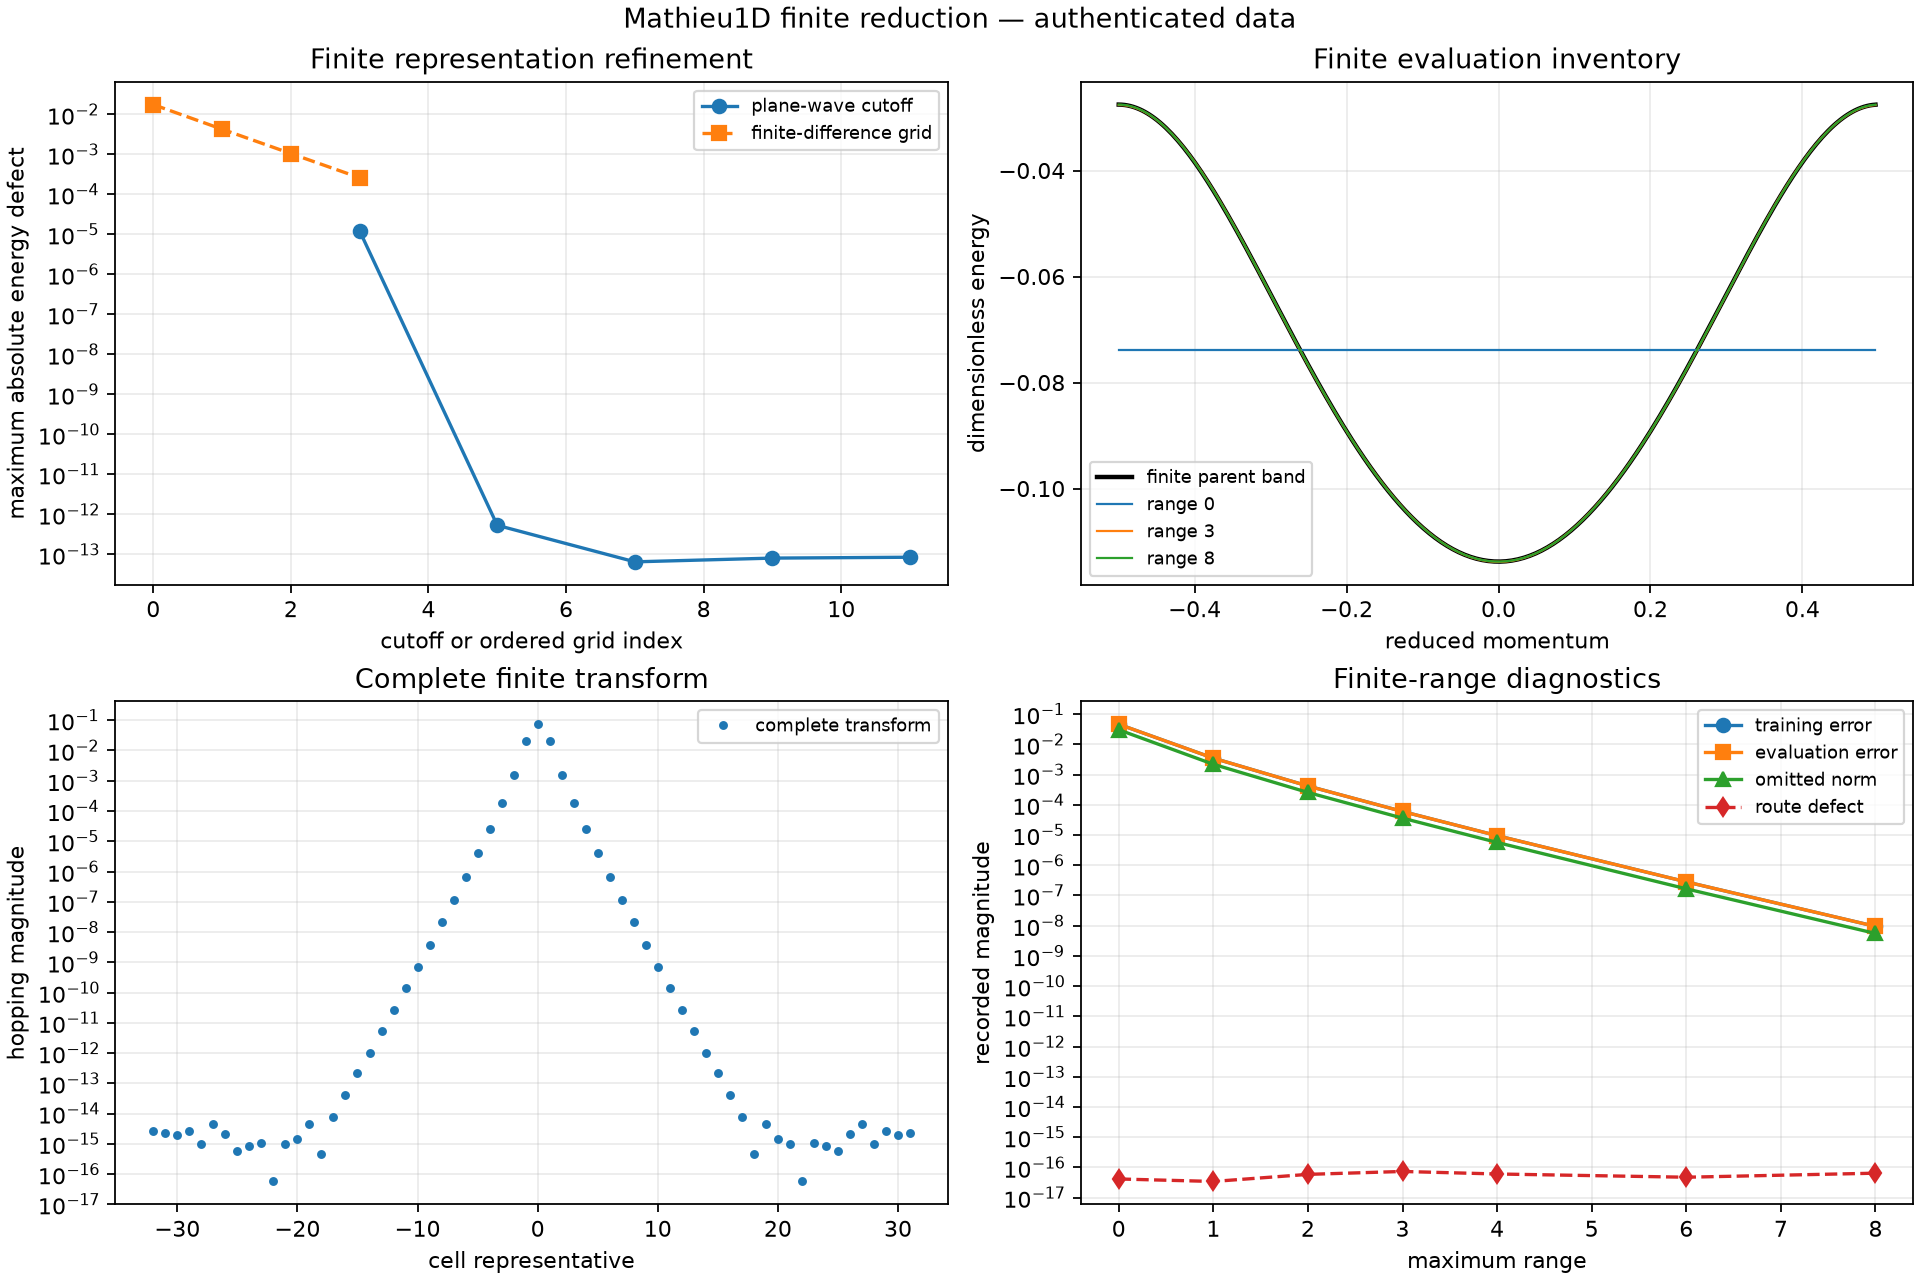
\includegraphics[width=\linewidth]{mathieu1d-finite-reduction.png}
\caption{Complete direct Mathieu1D visualization rendered from the independently
verified typed projection.}
\label{fig:complete}
\end{figure}

\section{Publication-facing finite-range summary}

Figure~\ref{fig:summary} is a compact projection of the same authenticated data.  Its
left panel records training and disjoint-evaluation maximum errors for every declared
range.  Its right panel records the corresponding omitted-block norm.  The compact
layout creates no new scientific values and is not an additional calculation.

\begin{figure}[htbp]
\centering
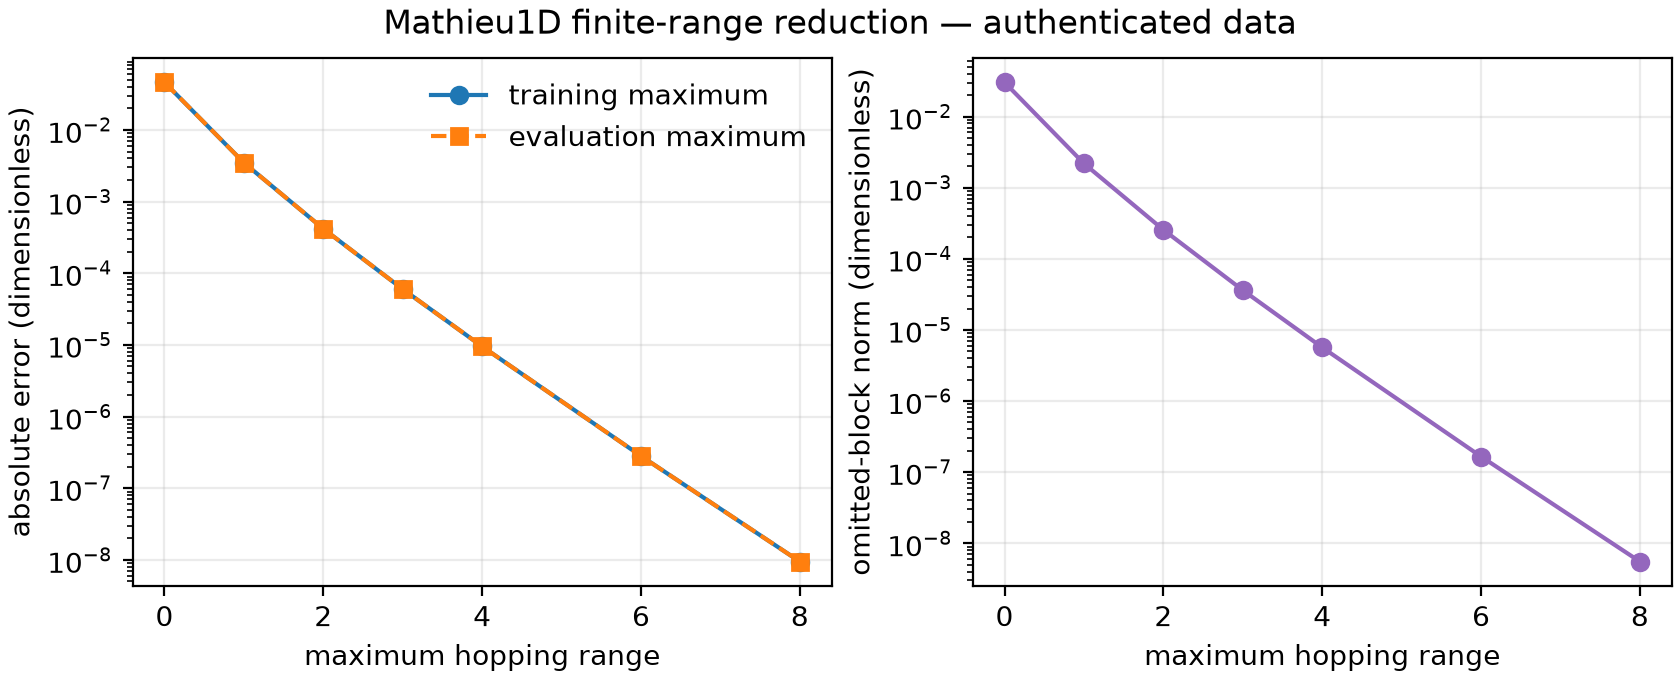
\includegraphics[width=0.97\linewidth]{mathieu1d-publication-summary.png}
\caption{Compact finite-range summary derived from the same authenticated projection
as Figure~\ref{fig:complete}.}
\label{fig:summary}
\end{figure}

\section{Interpretation limits}

The plane-wave reference is itself finite.  The finite-difference sequence is a
comparison among represented matrices, not a certified continuum enclosure.  The
complete discrete transform reconstructs one finite sampled inventory; truncating it
tests declared finite model classes.  Agreement between the mediated and direct-fit
routes is meaningful only under the matched coordinates, weights, and model class used
here.  Sampled band gaps do not certify continuum spectral isolation, and no hopping
range is accepted as universally adequate.

The present direct execution is the sole live Mathieu1D calculation and publication
source.  Predecessor code and run artifacts are absent from the live tree and are not
runtime, verification, rendering, or report inputs.

\end{document}
